\setcounter{chapter}{10}  % sets the current chapter to 10 so that the next one becomes 11

\chapter{Introduction to Hypothesis Testing}
\label{ch:intro-hypothesis}

\section{Test of Hypothesis for One Mean}

\begin{definition}[Hypothesis Tests]
An inferential procedure to determine whether there is sufficient evidence to suggest a condition for a population parameter using statistics from a sample.
\end{definition}


\textcolor{blue}{Attach a probability to the conclusion of a hypothesis test.}

\subsubsection*{Steps}
\begin{enumerate}
    \item Decide on a level of significance ($\alpha$)
    \item State the null hypothesis ($H_0$) and the alternative hypothesis ($H_a$) \textcolor{blue}{($H_1$)}
    \item Calculate the appropriate test statistic.
    \item Use the test statistic and a reference distribution to calculate a p-value. \\
    \textcolor{blue}{(Also refer back to $H_a$)}
    \item Compare p-value to $\alpha$ to make a conclusion.
\end{enumerate}

\textcolor{blue}{Note:} \\
\textcolor{blue}{The definition of a p-value can be confusing. We will define it later.}

\subsection*{Step 1: Decide on a Level of Significance ($\alpha$)}
-Threshold for decision making.

-Depends on tolerance for consequences of errors, sample size, nature of the study, and variability.

-Common values: $0.10$, $0.01$, $0.05$ \textcolor{blue}{(very common default)}

\subsection*{Step 2: State the Null Hypothesis ($H_0$) and the Alternative Hypothesis ($H_a$)}

\textbf{$\Theta$:} parameter of interest

\textbf{$\Theta_0$:} numerical value of the parameter of interest hypothesized under the null hypothesis.

\[
\begin{array}{lll}
H_0: \Theta = \Theta_0 & (\Theta \leq \Theta_0) & H_a: \Theta > \Theta_0 \quad \textcolor{blue}{\text{one-sided (one-tailed)}} \\
H_0: \Theta = \Theta_0 & (\Theta \geq \Theta_0) & H_a: \Theta < \Theta_0 \quad \textcolor{blue}{\text{one-sided (one-tailed)}} \\
H_0: \Theta = \Theta_0 &                         & H_a: \Theta \neq \Theta_0 \quad \textcolor{purple}{\text{two-sided (two-tailed)}}
\end{array}
\]


\textbf{Null ($H_0$):} Represents the current belief (\textcolor{blue}{status quo}) or the safe belief.

\textbf{Alternative ($H_a$):} Represents the research hypothesis (or what you are asked to test)
\subsection*{Step 3: Calculate an appropriate test statistic}

Depends on the hypothesis test conducted and the information available.


\begin{definition}[Test Statistic Skeleton]
\[
\text{test statistic} = \frac{\text{(a statistic)} - \text{(hypothesized value of parameters under } H_0 \text{)}}{\text{standard error of statistic}}
\]
\end{definition}

The test statistic follows a reference distribution ($Z$, $t$, $F$, $\chi^2$).
\subsection*{Step 4: Calculate the p-value}

\noindent
Use the test statistic, reference distribution, and refer back to $H_a$.

% --- BLUE: Right-tailed tests ---
\begin{figure}[H]
  \centering
  \begin{minipage}[t]{0.48\textwidth}
    \centering
    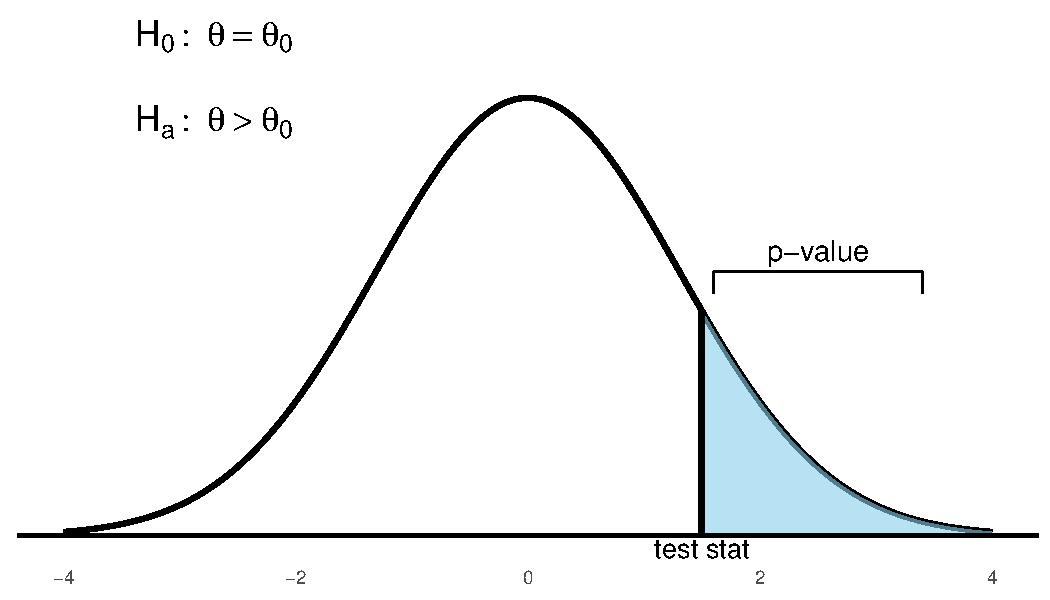
\includegraphics[width=\linewidth]{section11/images/hypothesis_right_tail.pdf}
  \end{minipage}
  \hfill
  \begin{minipage}[t]{0.48\textwidth}
    \centering
    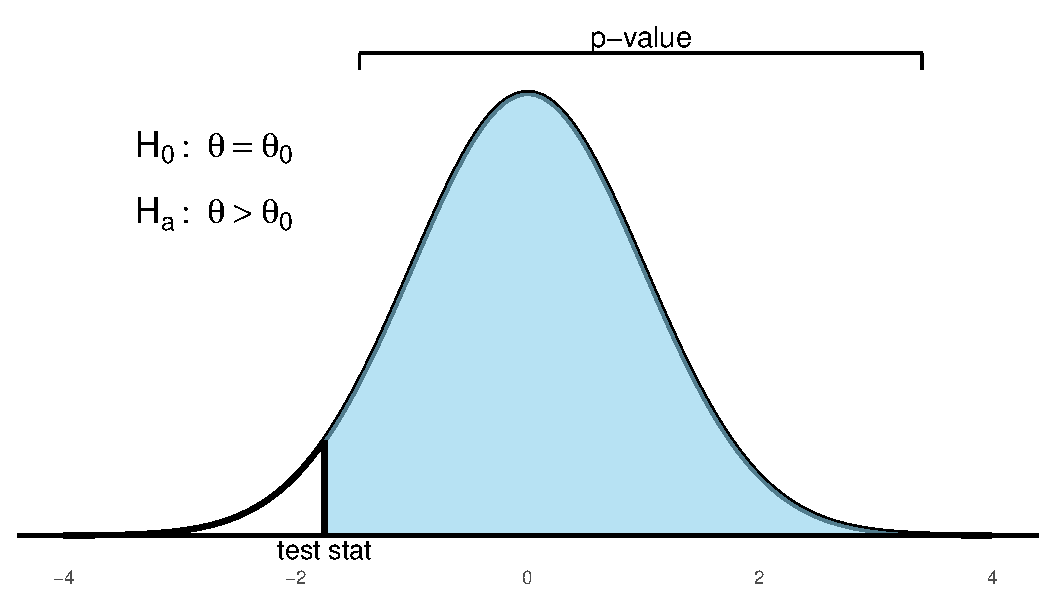
\includegraphics[width=\linewidth]{section11/images/hypothesis_right_tail_wide.pdf}
  \end{minipage}
  \caption*{Right-tailed test: \textit{p}-value is the area to the right of the test statistic.}
\end{figure}


% --- PINK: Left-tailed tests ---
\begin{figure}[H]
  \centering
  \begin{minipage}{0.48\textwidth}
    \centering
    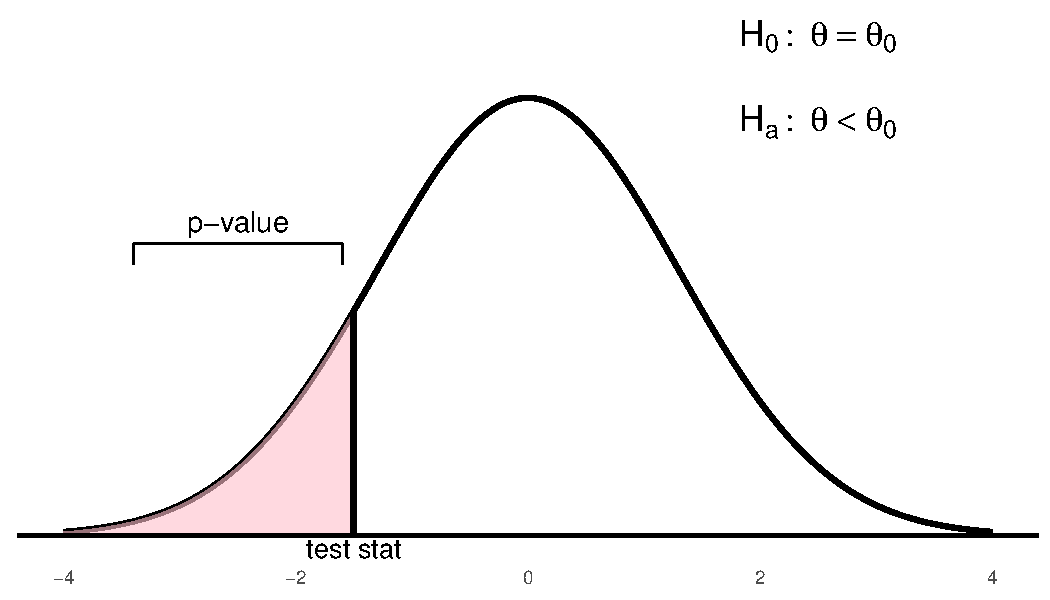
\includegraphics[width=\textwidth]{section11/images/hypothesis_left_tail.pdf}
  \end{minipage}
  \hfill
  \begin{minipage}{0.48\textwidth}
    \centering
    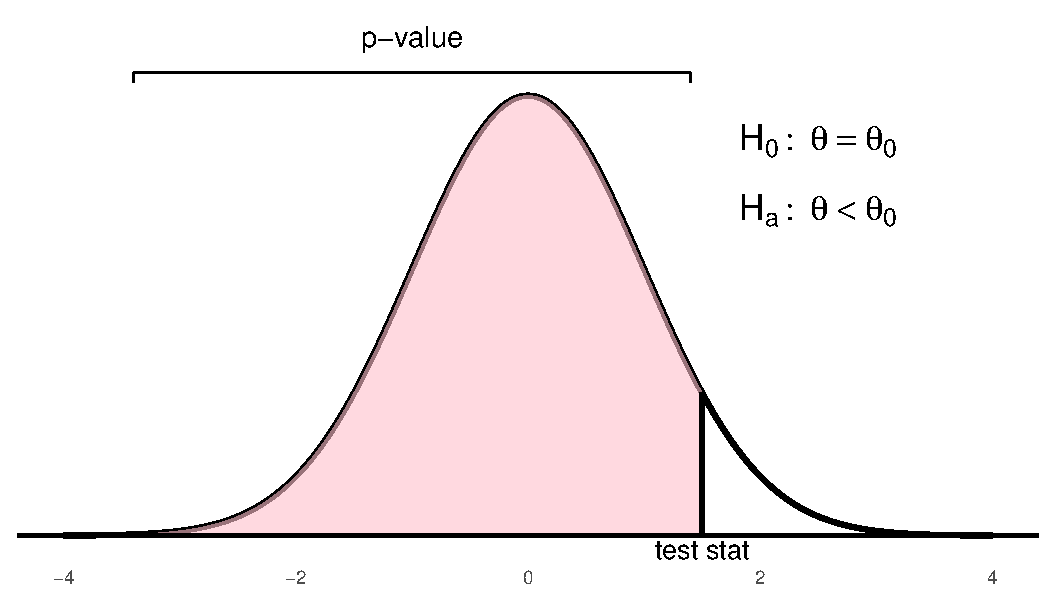
\includegraphics[width=\textwidth]{section11/images/hypothesis_left_tail_wide.pdf}
  \end{minipage}
\caption*{Left-tailed test: \textit{p}-value is the area to the left of the test statistic.}
\end{figure}

% --- GREEN: Two-tailed test ---
\begin{figure}[H]
  \centering
  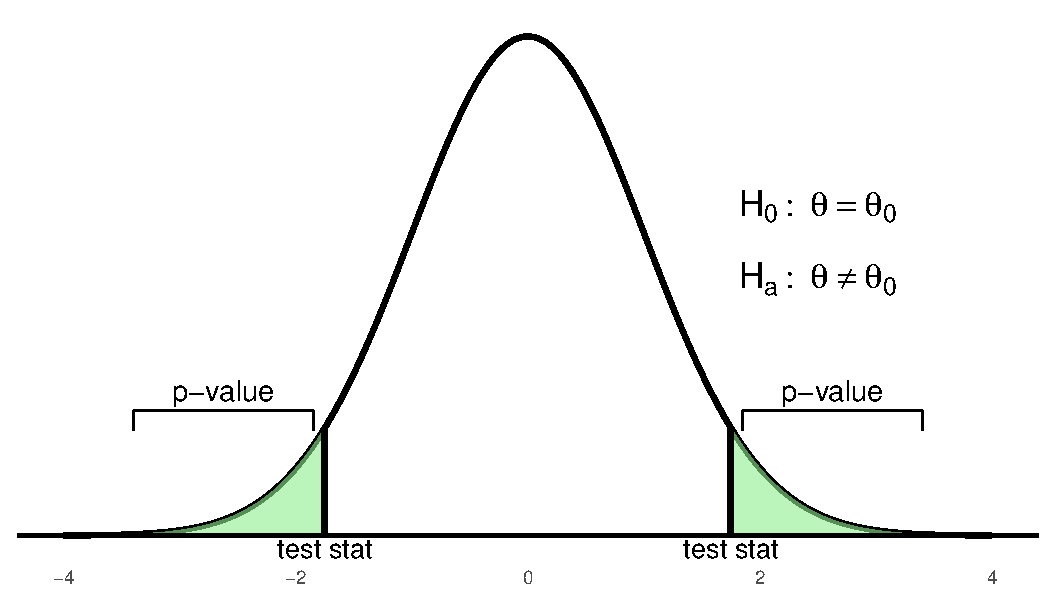
\includegraphics[width=0.52\textwidth]{section11/images/hypothesis_two_tail.pdf}
  \caption*{Two-tailed test: p-value is the total area in both tails beyond $\pm$ test statistic.}
\end{figure}
\subsection*{Step 5: Compare \textit{p}-value to level of significance $\alpha$ and make a conclusion}

\begin{itemize}
  \item If \textit{p}-value $< \alpha$: \\
  \quad Sufficient evidence against $H_0$. The hypothesis test rejects $H_0$ in favor of $H_a$.

  \item If \textit{p}-value $> \alpha$: \\
  \quad Insufficient evidence against $H_0$. Do not reject $H_0$ (fail to reject $H_0$).
\end{itemize}

\textbf{Note:} It is not good practice to give conclusions in the context of stating we \textit{accept $H_0$} or \textit{accept $H_a$}.
\begin{example}[Sweetening Colas]
Diet colas use artificial sweeteners to avoid sugar. These sweeteners gradually lose their sweetness over time. Manufacturers therefore test new colas for loss of sweetness before marketing them. Trained tasters sip the cola along with drinks of standard sweetness and score the cola on a “sweetness score” of 1 to 10. The cola is then stored for a month at high temperature to imitate the effect of four months’ storage at room temperature. Each taster scores the cola again after storage. This is a matched pairs experiment. Our data are the differences (score before storage minus score after storage) in the tasters’ scores. The bigger these differences, the bigger the loss of sweetness.

Suppose we know that for any cola, the sweetness loss scores vary from taster to taster according to a Normal distribution with standard deviation $\sigma = 1$. The mean $\mu$ for all tasters measures loss of sweetness.

The following are the sweetness losses for a new cola as measured by 10 trained tasters:

\medskip
\centerline{2.0,\ 0.4,\ 0.7,\ 2.0,\ -0.4,\ 2.2,\ -1.3,\ 1.2,\ 1.1,\ 2.3}
\medskip

Are these data good evidence that the cola lost sweetness in storage?\\
\noindent\textbf{Solution}\\

$\mu$ = mean sweetness loss for the population of \textbf{all} tasters.\\
\textbf{Step 1:} State hypotheses. $H_0: \mu = 0$ vs $H_a: \mu > 0$ \\
\textbf{Step 2:} Test statistic: $z_\star = \dfrac{\bar{x} - \mu_0}{\sigma / \sqrt{n}} = \dfrac{1.02 - 0}{1 / \sqrt{10}} = 3.23$ \\
\textbf{Step 3:} P-value. $P(Z > z_\star) = P(Z > 3.23) = 0.0006$ \\
\textbf{Step 4:} Conclusion. We would rarely observe a mean as large as 1.02 if $H_0$ were true. The small p-value provides strong evidence against $H_0$, supporting $H_a: \mu > 0$. That is, the mean sweetness loss is likely positive.

\vspace{1em}
\noindent\textbf{R code (Simulation)}

\begin{tcolorbox}[colback=gray!10, colframe=black!45, arc=2mm]
\begin{verbatim}
# n = sample size;
n<-10;
mu.zero<-0;
sigma<-1;
sigma.xbar<-sigma/sqrt(n);

# x bar = sample mean with 10 obs;
x.bar<-rnorm(1,mean=mu.zero,sd=sigma.xbar);
x.bar;

## [1] 0.3265859

# z.star = test statistic;
z.star<-(x.bar-mu.zero)/sigma.xbar;
z.star;

## [1] 1.032755
\end{verbatim}
\end{tcolorbox}
\vspace{1em}
\noindent\textbf{R code (10,000 Simulations)}

\begin{tcolorbox}[colback=gray!10, colframe=black!45, arc=2mm]
\begin{verbatim}
n <- 10;
mu.zero <- 0;
sigma <- 1;
sigma.xbar <- sigma / sqrt(n);
# x bar = sample mean with 10 obs;
# m = number of simulations;
m <- 10000;
x.bar <- rnorm(m, mean = mu.zero, sd = sigma.xbar);

# z.star = test statistic;
z.star <- (x.bar - mu.zero) / sigma.xbar;
hist(z.star, xlab = "differences", col = "blue");
\end{verbatim}
\end{tcolorbox}
\vspace{1em}
\noindent\textbf{Histogram from simulation (see Section 7 for R code format)}

\begin{figure}[H]
  \centering
  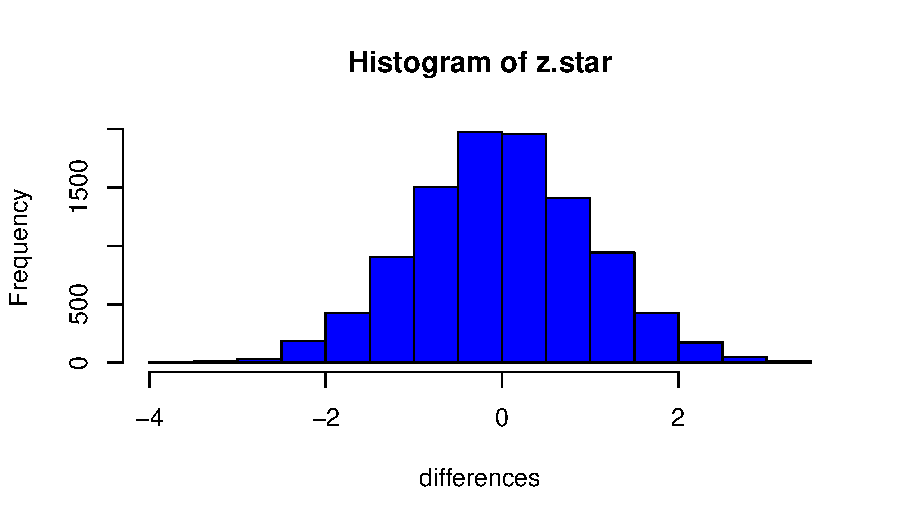
\includegraphics[width=0.6\textwidth]{Section11/images/sweetening_10000_hist.pdf}
  \caption*{Histogram of $z_\star$ values from 10,000 simulations under $H_0$.}
\end{figure}
\vspace{1em}
\noindent\textbf{R code (Empirical p-value)}

\begin{tcolorbox}[colback=gray!10, colframe=black!45, arc=2mm]
\begin{verbatim}
## P-value

p_value <- length(z.star[z.star > 3.23]) / m;

p_value

## [1] 8e-04
\end{verbatim}
\end{tcolorbox}


\end{example}




